% =============================================================
% Supplementary material (draft) -- DINOcow paper
% =============================================================
\clearpage
\section*{Supplementary material}
\cajanueva{\textit{Baselines, training behavior and DINOcow error}}\par\medskip
\setcounter{table}{0}\setcounter{figure}{0}
\renewcommand{\thetable}{S\arabic{table}}\renewcommand{\thefigure}{S\arabic{figure}}

Table~\ref{tab:S1} extends Table~\ref{tab:summary}, with predictions averaged over the three seeds. Bias is the mean signed error for thin ($<3$) and fat ($\geq4.5$) cows.

\begin{table}[!htbp]
  \centering
  \caption{Detailed comparison with the baselines on unseen cows (five cow-level folds $\times$ 3 seeds).}
  \label{tab:S1}
  \resizebox{\textwidth}{!}{%
  \cajanueva{\begin{tabular}{lcccccccc}
    \toprule
    Method & MAE $\downarrow$ & RMSE $\downarrow$ & $R^2$ $\uparrow$ & $\pm0.5$ $\uparrow$ & MAE/cow $\downarrow$ & $\Delta$ MAE/cow [95\% CI] $\downarrow$ & Bias thin $\to0$ & Bias fat $\to0$ \\
    \midrule
    \textbf{DINOcow (our model)} & \textbf{0.428} & \textbf{0.537} & \textbf{0.70} & \textbf{75\%} & \textbf{0.414} & -- & \textbf{+0.53} & \textbf{$-$0.29} \\
    DINOcow, 80\% of training cows & 0.438 & 0.544 & \textbf{0.70} & 72\% & 0.424 & +0.010 [$-$0.003, +0.024] & +0.54 & $-$0.33 \\
    DINOv3 + LoRA, regions & 0.433 & 0.539 & \textbf{0.70} & \textbf{75\%} & 0.428 & +0.014 [$-$0.018, +0.046] & +0.57 & $-$0.35 \\
    DINOv3 + LoRA & 0.437 & 0.557 & 0.68 & \textbf{75\%} & 0.434 & +0.020 [$-$0.025, +0.066] & +0.57 & $-$0.35 \\
    ResNet-50, fine-tuned & 0.656 & 0.795 & 0.35 & 58\% & 0.614 & +0.200 [+0.131, +0.270] & +1.06 & $-$0.53 \\
    EfficientNet-V2-S, fine-tuned & 0.639 & 0.759 & 0.41 & 55\% & 0.625 & +0.211 [+0.152, +0.272] & +0.98 & $-$0.60 \\
    ViT-B/16, fine-tuned & 0.660 & 0.811 & 0.32 & 53\% & 0.628 & +0.215 [+0.152, +0.282] & +0.98 & $-$0.60 \\
    ResNet-50, frozen + ridge & 0.652 & 0.805 & 0.34 & 55\% & 0.642 & +0.228 [+0.165, +0.293] & +0.86 & $-$0.68 \\
    EfficientNet-B0, fine-tuned & 0.726 & 0.880 & 0.21 & 50\% & 0.667 & +0.253 [+0.179, +0.331] & +1.22 & $-$0.65 \\
    YOLO11s-cls & 0.740 & 0.903 & 0.16 & 47\% & 0.707 & +0.293 [+0.211, +0.381] & +1.14 & $-$0.73 \\
    YOLOv8s-cls & 0.775 & 0.907 & 0.16 & 41\% & 0.713 & +0.299 [+0.220, +0.384] & +1.05 & $-$0.86 \\
    \bottomrule
  \end{tabular}}}
\end{table}

\begin{figure}[!htbp]
  \centering
  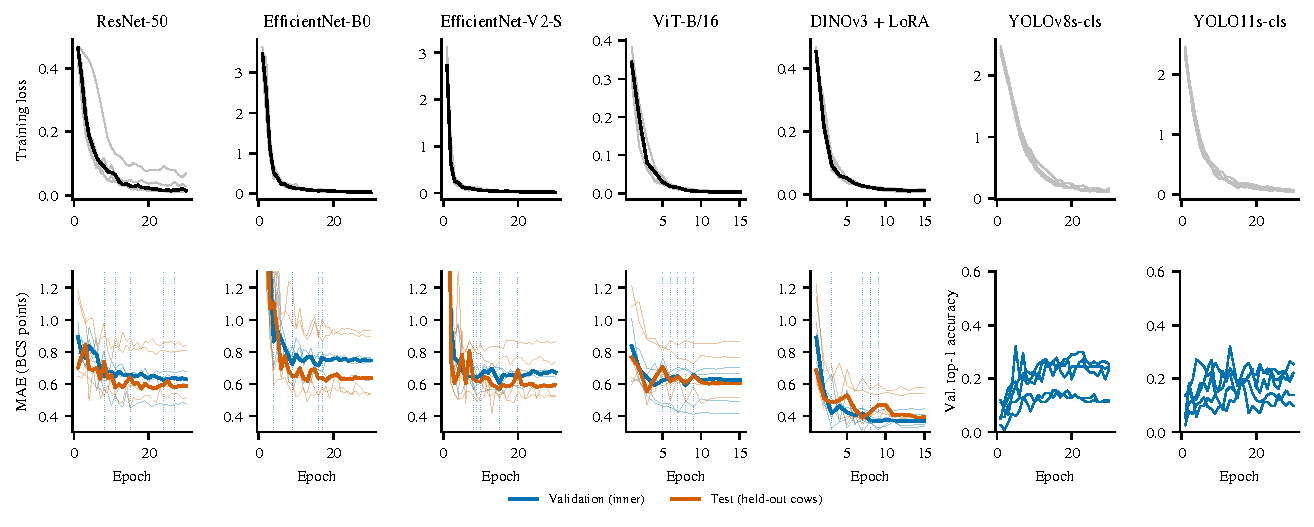
\includegraphics[width=\textwidth]{../figures/curvas_entrenamiento.pdf}
  \caption{Training curves of the fine-tuned baselines (seed 0). Top, training loss. Bottom, validation and test error.}
  \label{fig:S1}
\end{figure}

\begin{figure}[!htbp]
  \centering
  \cajanueva{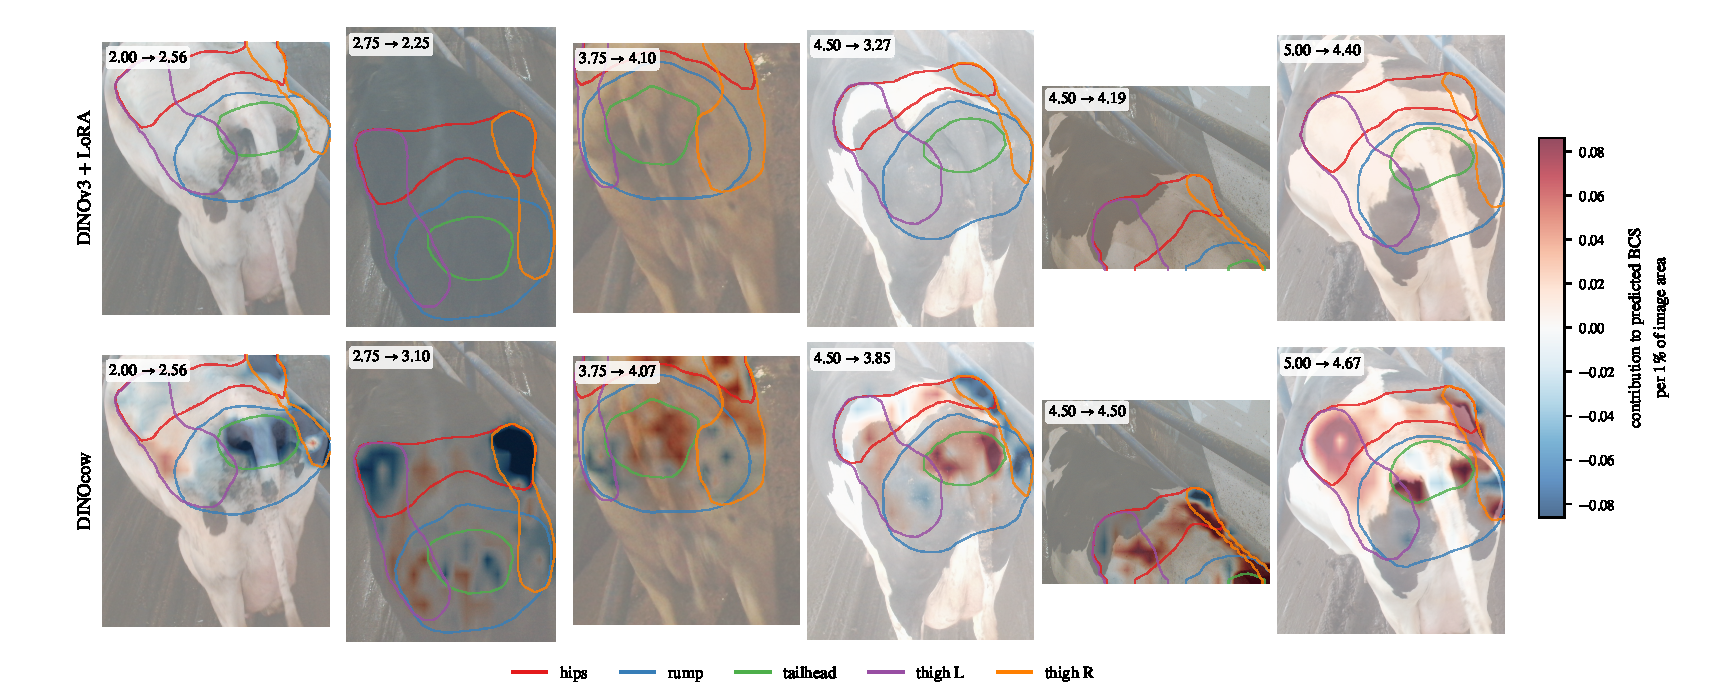
\includegraphics[width=0.97\textwidth]{../figures/comparacion_mapas.pdf}}
  \caption{Contribution of each image patch to the predicted BCS for DINOv3 with LoRA (top) and DINOcow (bottom), on test cows of one fold ordered by reference score. Each panel gives the reference and predicted BCS.}
  \label{fig:S2}
\end{figure}

\pendiente{Fig.~S3: MAE per cow against DINOv3 block (sweep over blocks 17--24).}

\begin{figure}[!htbp]
  \centering
  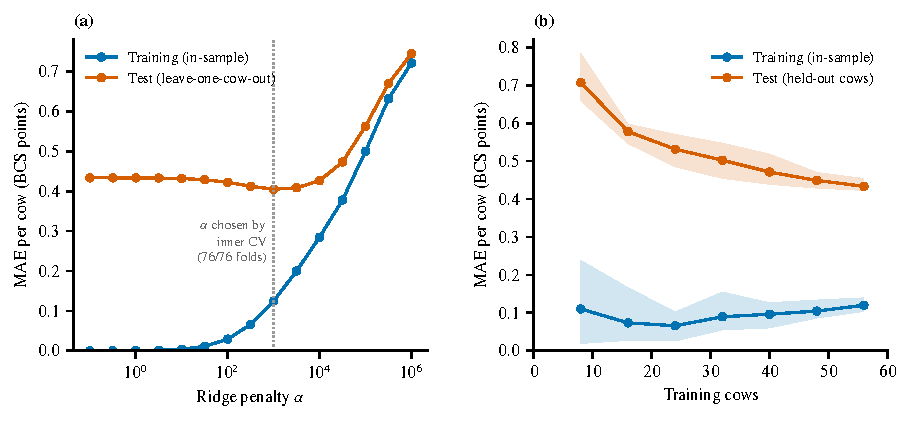
\includegraphics[width=\textwidth]{../figures/curvas_modelo.pdf}
  \caption{Error of DINOcow. (a) MAE per cow against the ridge penalty $\alpha$. (b) Training and test MAE per cow against the number of training cows.}
  \label{fig:S4}
\end{figure}
